% auto-generated by scripts/pilot_design_stdlib.py（標準ライブラリ・勾配ロジスティック）
% sklearn 環境では \texttt{python -m analytics.pilot\_design\_analysis} で図付きに置き換え可
\begin{table}[htbp]
  \centering
  \small
  \caption{パイロット候補の記述（\texttt{recency}, \texttt{history}, \texttt{used\_discount}, \texttt{used\_bogo}, \texttt{is\_referral}, \texttt{zip\_code} のみから勾配ロジスティックでスコア化し上位\%で定義。演習用）}
  \label{tab:pilot_cohort}
  \begin{tabular}{@{}lrrrr@{}}
    \toprule
    セグメント & $n$ & CVR & mean(history) & mean(recency) \\
    \midrule
    全体 & 64000 & 0.1468 & 242.09 & 5.76 \\
    上位10\% & 6400 & 0.2500 & 515.85 & 2.75 \\
    上位5\% & 3200 & 0.2678 & 599.14 & 2.53 \\
    \bottomrule
  \end{tabular}
\end{table}

\begin{table}[htbp]
  \centering
  \small
  \caption{上位10\%コホート内の観察オファー別CVR（割当交絡あり・記述）}
  \label{tab:pilot_obs_offer}
  \begin{tabular}{@{}lrrr@{}}
    \toprule
    offer & $n$ & CVR \\
    \midrule
    Discount & 2172 & 0.2983 \\

    Buy One Get One & 2100 & 0.2476 \\

    No Offer & 2128 & 0.2030 \\

    \bottomrule
  \end{tabular}
\end{table}

\begin{figure}[htbp]
  \centering
  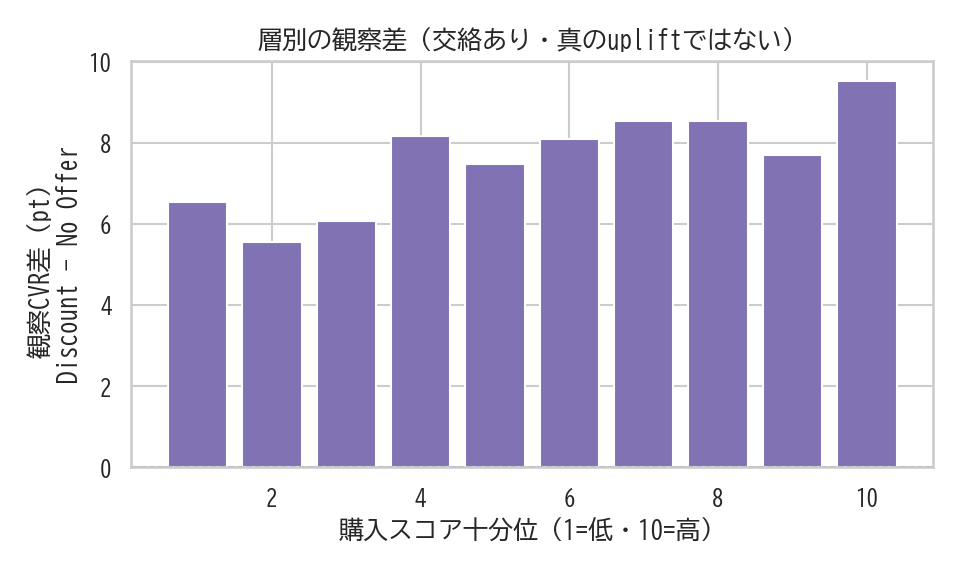
\includegraphics[width=0.88\linewidth]{../figures/improvements/uplift_crude_gap_by_score_decile.png}
  \caption{購入スコア（本スクリプトの6次元ロジスティック）十分位ごとの\textbf{観察}CVR差（Discount $-$ No Offer）。\textbf{割当は無作為ではない}ため真の増分（uplift）ではない。高スコア側で差が相対的に小さい層がありうる――\textbf{無駄割引}仮説の動機付けとして参照し、RCTで検証する。}
  \label{fig:uplift_crude_gap}
\end{figure}

\begin{table}[htbp]
  \centering
  \small
  \caption{仮定MDE（絶対差）に対する片群必要人数の目安（ベースラインCVR$=$25.00\%、上位10\%コホート。二比例・$\alpha$=0.05・正規近似）}
  \label{tab:pilot_power}
  \begin{tabular}{@{}rrrr@{}}
    \toprule
    MDE（絶対差） & 検定力 & 片群$n$（近似） & 3臂合計$n$目安 \\
    \midrule
    0.010 & 0.8 & 29821 & 89463 \\

    0.010 & 0.9 & 39921 & 119763 \\

    0.020 & 0.8 & 7550 & 22650 \\

    0.020 & 0.9 & 10107 & 30321 \\

    \bottomrule
  \end{tabular}
\end{table}